\documentclass[12pt,a4paper]{article}
\usepackage{graphicx}
\usepackage{amsmath}

\usepackage[backend=biber]{biblatex} 
\addbibresource{data.bib}

\begin{document}
\begin{titlepage}
	\centering
	{\scshape\LARGE Yale University \par}
	\vspace{1cm}
	{\scshape\Large Senior Thesis for the Mathematics and Computer Science major\par}
	\vspace{1.5cm}
	{\huge\bfseries Recurrent Neural Networks for Change Point Analysis\par}
	\vspace{2cm}
	{\Large\itshape William Cai\par}
	\vfill
	supervised by\par
	Prof.~Sahand \textsc{Negahban}

	\vfill

% Bottom of the page
	{\large \today\par}
\end{titlepage}
\begin{abstract}
In this paper we present a synthetic time-series dataset which is motivated by vital measurements for patients in the ICU (MIMIC).  At time zero, the time series moves according to one probability distribution.  We then have some criterion (motivated by events such as cardiac arrest), which a fraction of the generated examples trigger, causing the probability distribution to change for the remainder of the time series.  We then try to solve the problems of regression, predicting what the next measurement will be, and classification, predicting which generation function is currently generating the data, on this dataset.  The models we consider include a random forest, single-layer perceptron, deep neural network, and a recurrent neural network.  We give a comparison of the capability of these models to do this kind of change point analysis, and also consider their robustness in the face of missing data.  
\end{abstract}

\section{Introduction}

-> Lot of interesting data is in time series (cite MIMIC)

-> RNNs are really powerful for time series (cite GRAVES, http://karpathy.github.io/2015/05/21/rnn-effectiveness/)

-> Lot of interesting time series have their distributions change at some point (cite DYNACARE)

-> Question: Can we use recurrent neural nets in time distributions with change points?  

\section{Data}
Our synthetic data takes the form of a n x T x d matrix where n is the number of patients, T is the number of measurements, and d is the dimensionality of the measurements.  \\

Before we begin generating the data, we initialize d x d matrices A and B which have 2-norm .9 and are rank 2.  We also initialize betashift, a d-dimensional vector where each entry is drawn from a normal distribution with mean 0 and variance 1 and normalized by $\sqrt{d}$.  Then, the synthetic data for each patient is generated as follows:\\

$P$, the data for a single patient, is a T x d matrix.  Let $P_i$ be the measurement of that patient at time $i$.  \\
$P_0$ is randomly initialized with all values drawn from a normal distribution with mean 0 and variance 1 and normalized by $\sqrt{d}$. \\
Then, $P_{t+1} = (1_AA+(1-1_A)B)P_{t} + \sigma_w \epsilon$ where: \\

$\sigma_w$ is set to .2 \\

$\epsilon$ is d-dimensional white noise with all values mean 0 variance 1\\

$1_A$ is an indicator variable which is 1 if there is no $i \leq t$ s.t. $P_i \cdot $ betashift $> .5$\\

To feed our data into our models, we use the window technique.  This means that each sample contains measurements from time $i$ to time $i + x - 1$, where $x$ is our window size.  For the models besides the recurrent neural net, this data is flattened into a vector of length $xd$, while recurrent neural networks take the data as an $x$ by $d$ matrix.  For regression this is regressed against the measurement at time $i + x$, and for classification we want to do binary classification on the value of $1_A$ at time $i + x$.  Our generated examples were split 80-20 into the training and validation sets.  

\section{Models}
\subsection{Random Forests}
We used scikit-learn's RandomForestRegressor and RandomForestClassifier.  We set the forest to have 40 estimators and features, except when the window only contained one set of measurements when we set it to 10 estimators.  

\subsection{Neural Network}
Our Neural Networks were built with Keras.  We used a single layer perceptron with 512 nodes using the rectified linear unit (ReLU) activator, with a dropout of .25.  For regression, the neural network feeds into a layer of d nodes, which is the dimensionality of the measurements we are trying to predict.  For classification it feeds into a single node which is converted to a classification using the sigmoid activation.  

\subsection{Deep Neural Network}
We used a two layer perceptron where each layer consisted of 512 nodes using the rectified linear unit (ReLU) activator, with a dropout of .25.  Again, for regression this feeds into a layer of d nodes and for classification it feeds into a single node which is converted to a classification using the sigmoid activation.  

\subsection{Recurrent Neural Network}
We used a 16 node Gated Recurrent Unit using the rectified linear unit (ReLU) activator which fed into a perceptron with 128 nodes and a dropout of .5 which also used the rectified linear unit (ReLU) activator.  Again, for regression this feeds into a layer of d nodes and for classification it feeds into a single node which is converted to a classification using the sigmoid activation.  

\section{Experiment}
There are two prediction problems we are interested in: 

1) Given $P_0$ through $P_t$, predict $P_{t+1}$ (regression). 

2) Given $P_0$ through $P_t$, predict $1_A$ (binary classification) 

\subsection{Regression}
Given a time series of measurements, we would like to be able to predict what the next measurement will be.  For this entire section, we let the dimensionality $d$ of the data be 10, the number of timesteps per patient $T$ be 175, and the number of patients $N$ to be 200.   First, we see how the models perform in the absence of the change point as a baseline.  Then, we see how the models perform on the data which has change points. For each model, we show the model's predictions for a patient in the validation set and give the best MSE achieved by that model.  Then, at the end of this section, we give a comparison of the models over various values of window size $x$.  

\subsection{Regression Baseline (no change points)}
As a baseline, we check to see how our models work when A = B, or in other words, the patient measurements are generated by: 
$$P_{t+1} = AP_{t} + \sigma_w \epsilon$$
In this case, the 'correct' model should predict $P_{t + 1} = AP_t$.  We can actually calculate the MSE that this model would give, which comes out to 0.1599351.  

\subsubsection{Random Forest Regression}
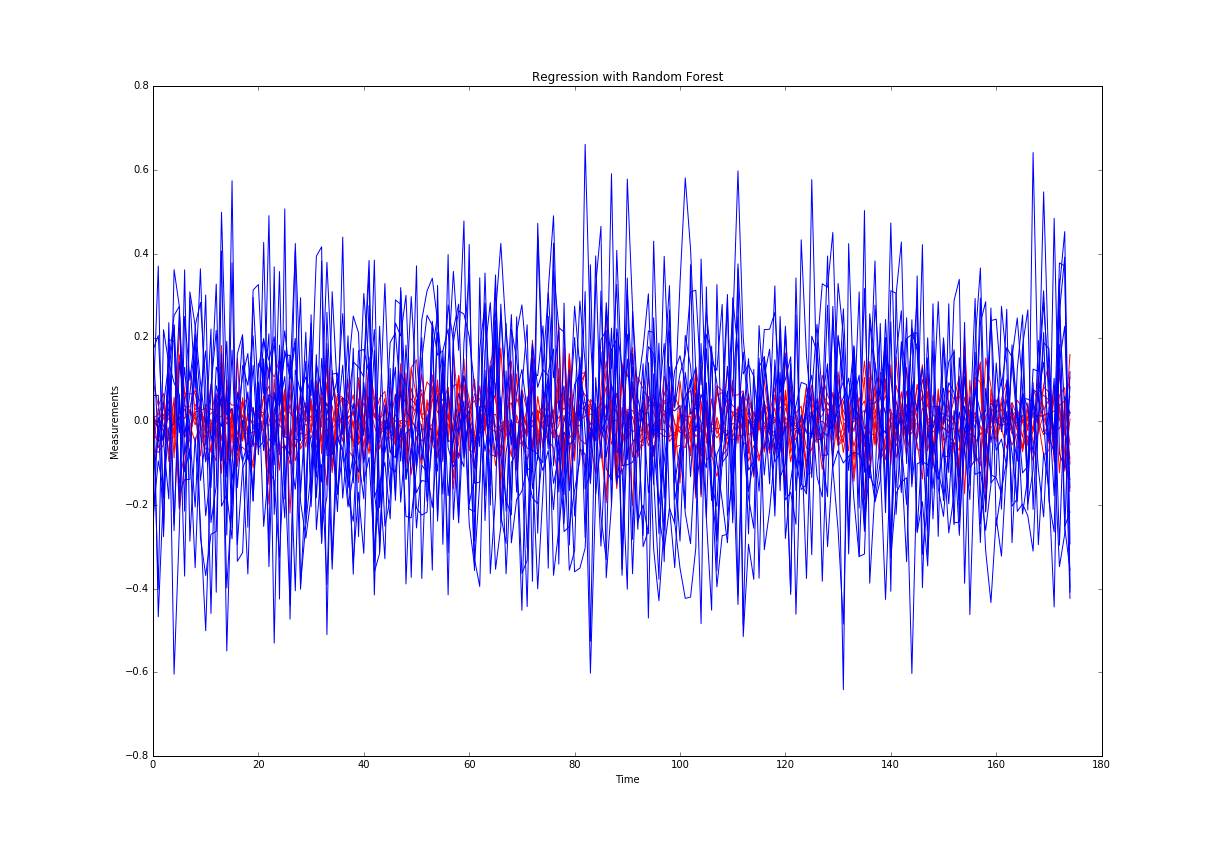
\includegraphics[height=200px, width=1\textwidth]{tree_regression_projection_a_eq_b}
MSE: 0.163457677349 \\
\subsubsection{Neural Network}
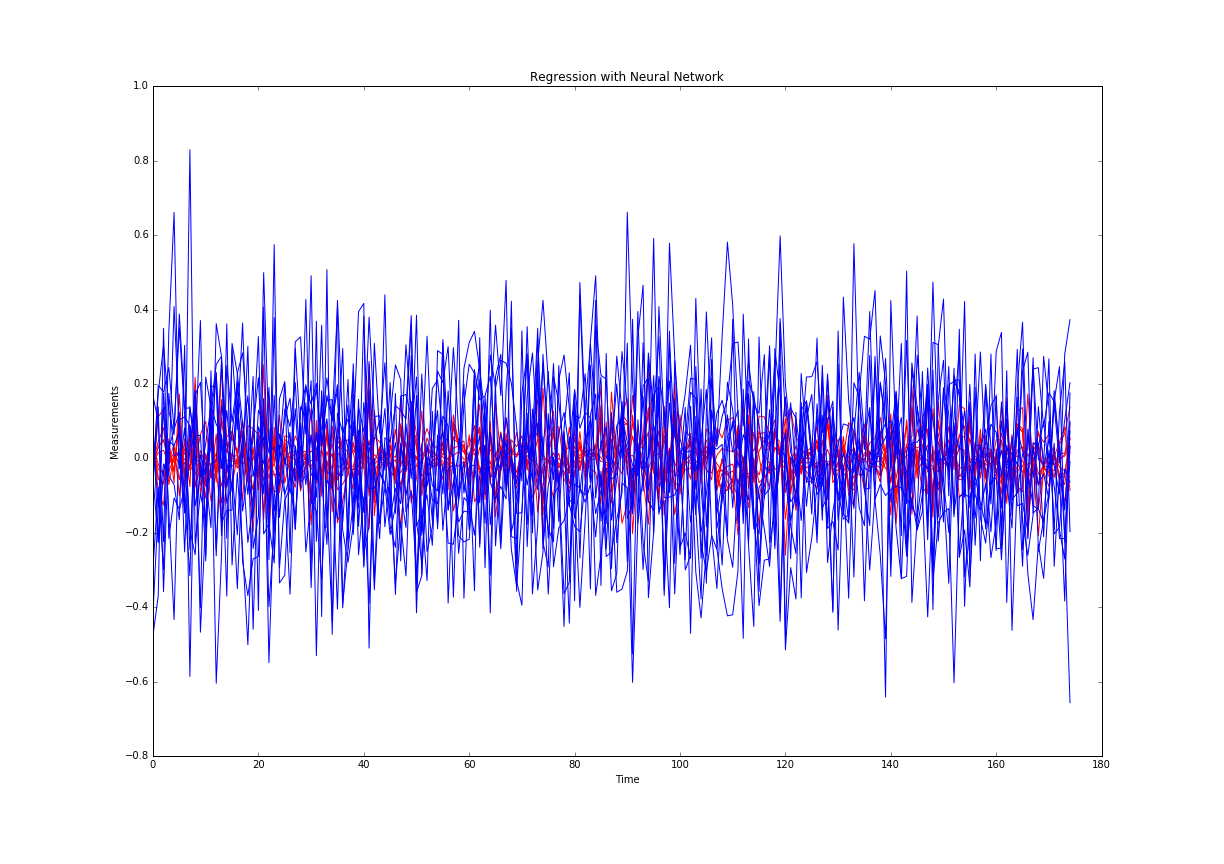
\includegraphics[height=200px, width=1\textwidth]{nn_regression_projection_a_eq_b}
MSE: 0.160142227167 \\
\subsubsection{Deep Neural Network}
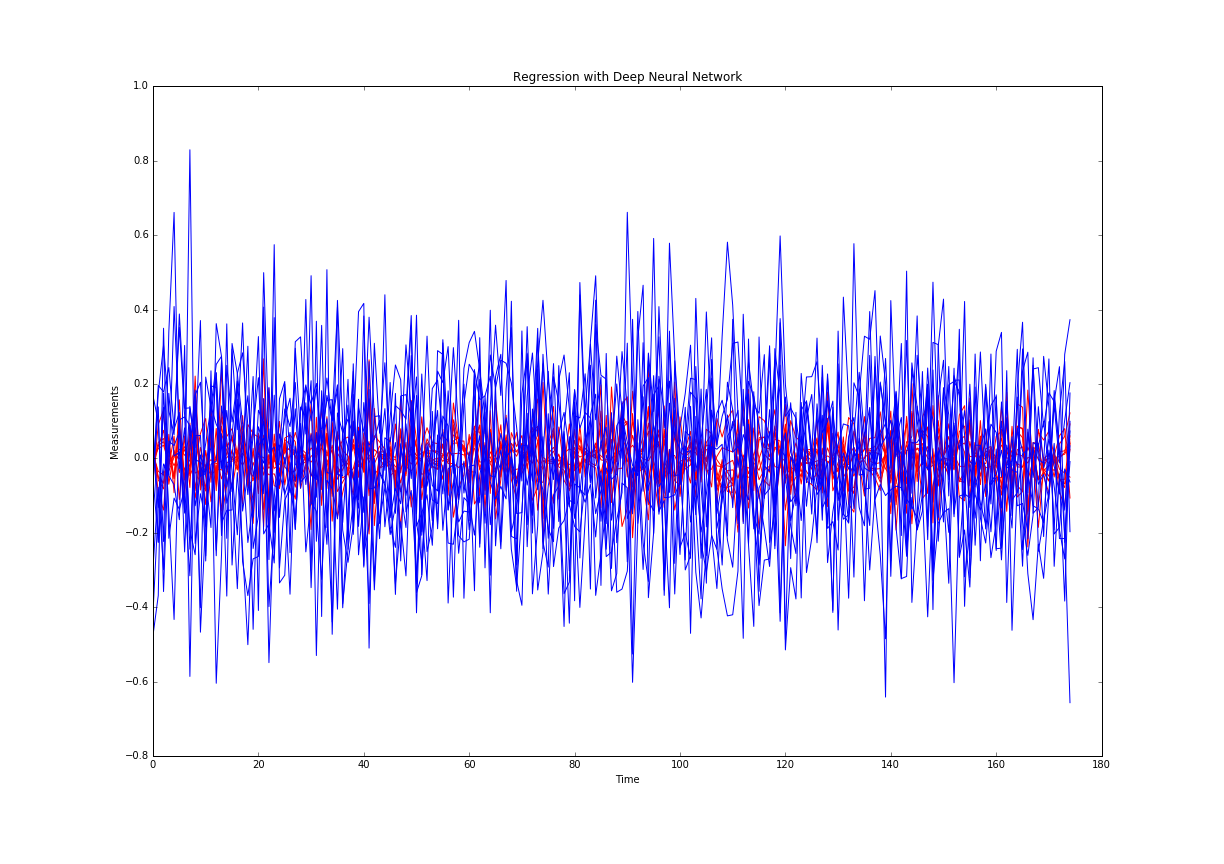
\includegraphics[height=200px, width=1\textwidth]{deep_nn_regression_projection_a_eq_b}
MSE: 0.160053838298 \\
\subsubsection{Recurrent Neural Network, window method}
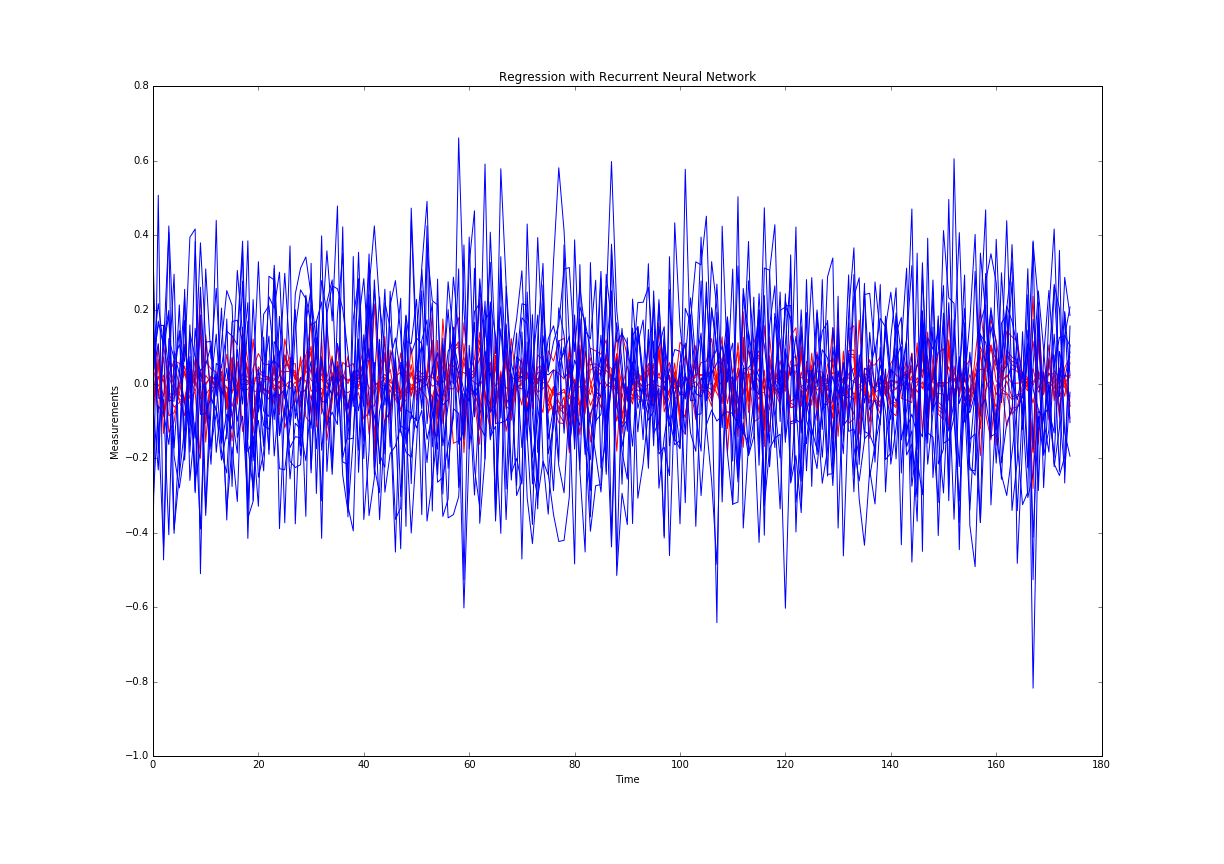
\includegraphics[height=200px, width=1\textwidth]{window_rnn_regression_projection_a_eq_b}
MSE: 0.159979021872 \\

\subsection{Regression (with change points)}

\subsubsection{Random Forest Regression}
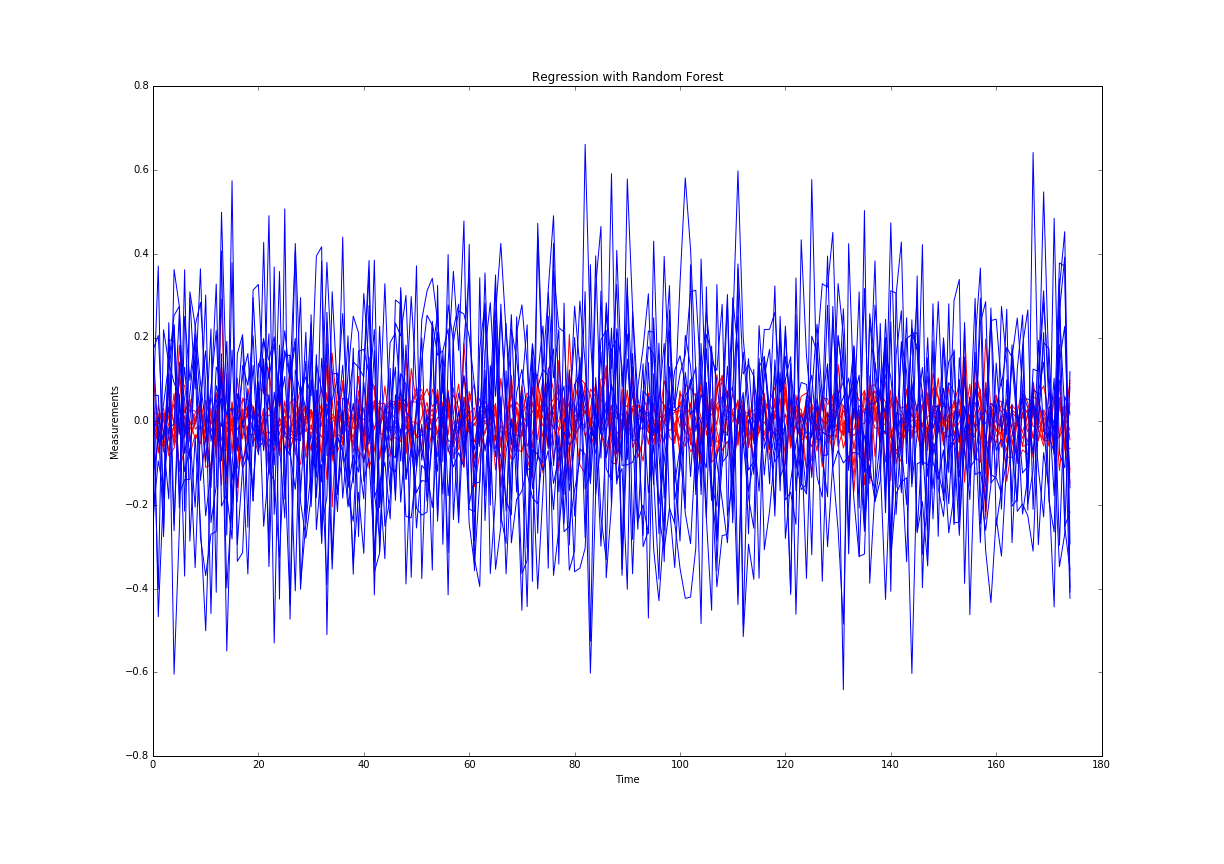
\includegraphics[height=200px, width=1\textwidth]{tree_regression_projection_a_neq_b}
We used scikit-learn's RandomForestRegressor, trained with 40 estimators and features, except when we were using a sequence length of 1, in which case we only used 10.  

\subsubsection{Neural Network}
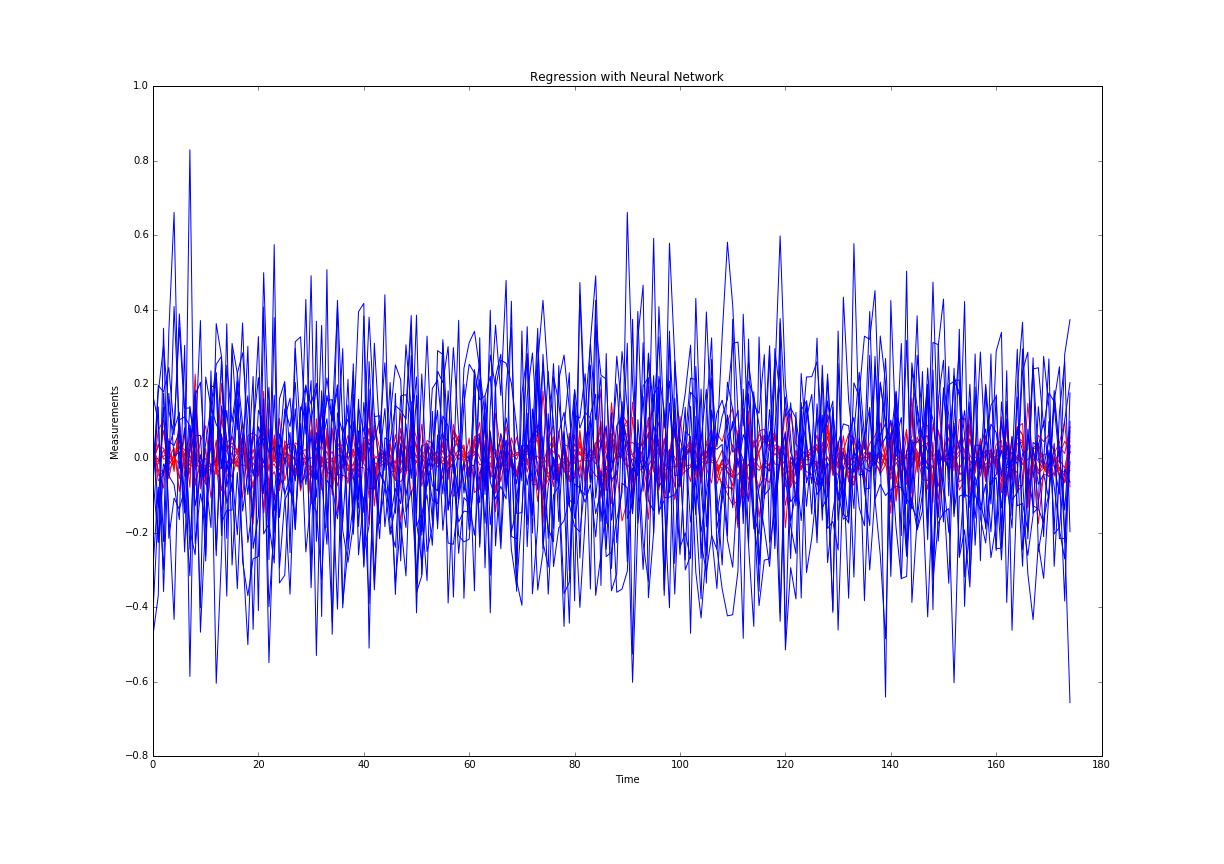
\includegraphics[height=200px, width=1\textwidth]{nn_regression_projection_a_neq_b}
We used a single layer perceptron with 512 nodes using the rectified linear unit (ReLU) activator, with a dropout of .25.  

\subsubsection{Deep Neural Network}
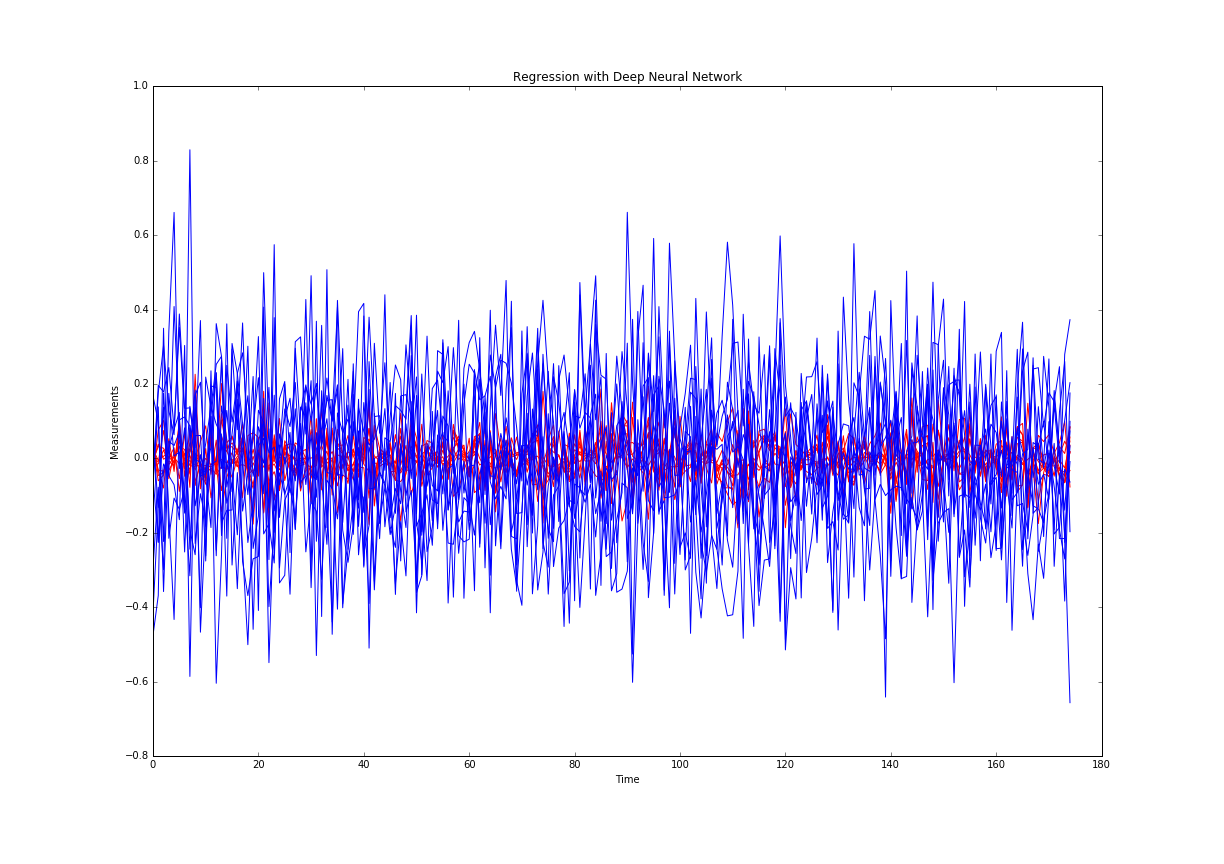
\includegraphics[height=200px, width=1\textwidth]{deep_nn_regression_projection_a_neq_b}
We used a two layer perceptron where each layer consisted of 512 nodes using the rectified linear unit (ReLU) activator, with a dropout of .25.  

\subsubsection{Recurrent Neural Network, window method}
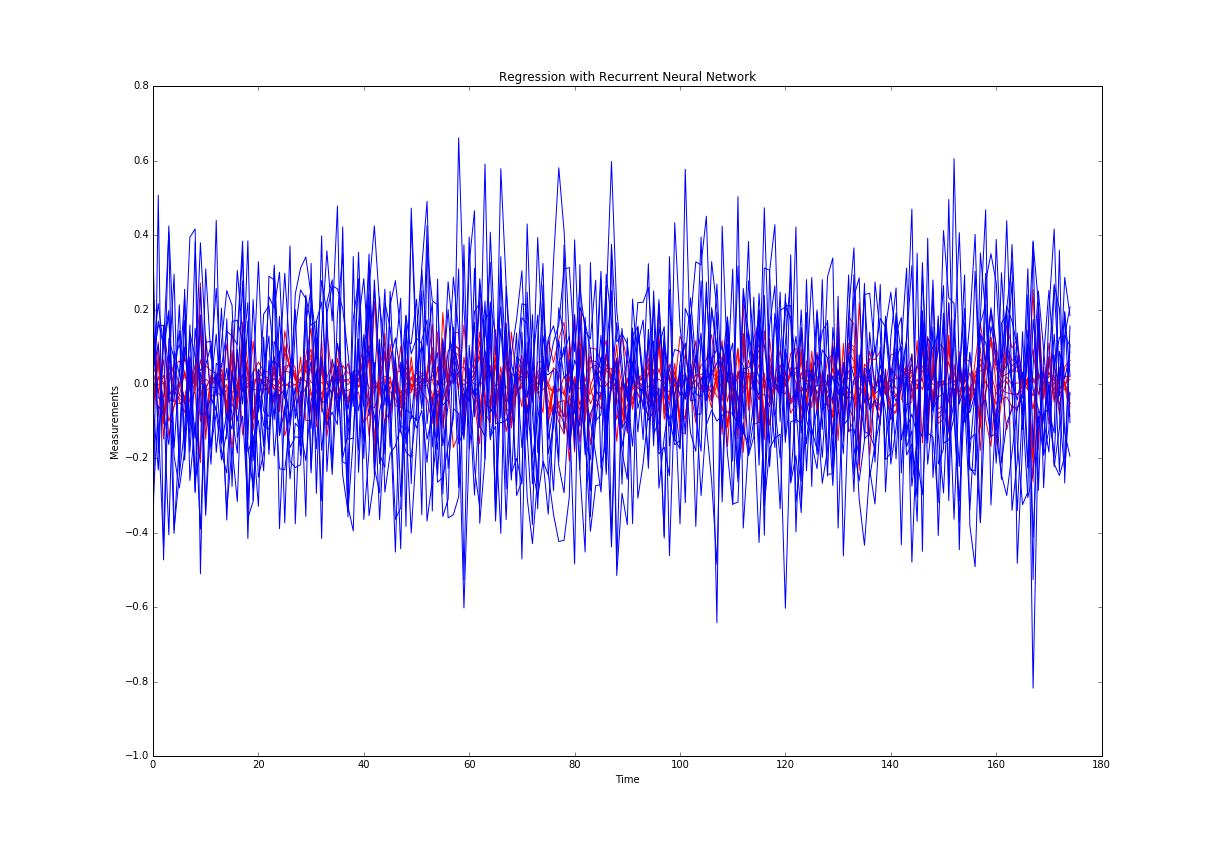
\includegraphics[height=200px, width=1\textwidth]{window_rnn_regression_projection_a_neq_b}
We used a 16 node Gated Recurrent Unit using the rectified linear unit (ReLU) activator which fed into a perceptron with 128 nodes and a dropout of .5 which also used the rectified linear unit (ReLU) activator.  

\subsubsection{Comparison}
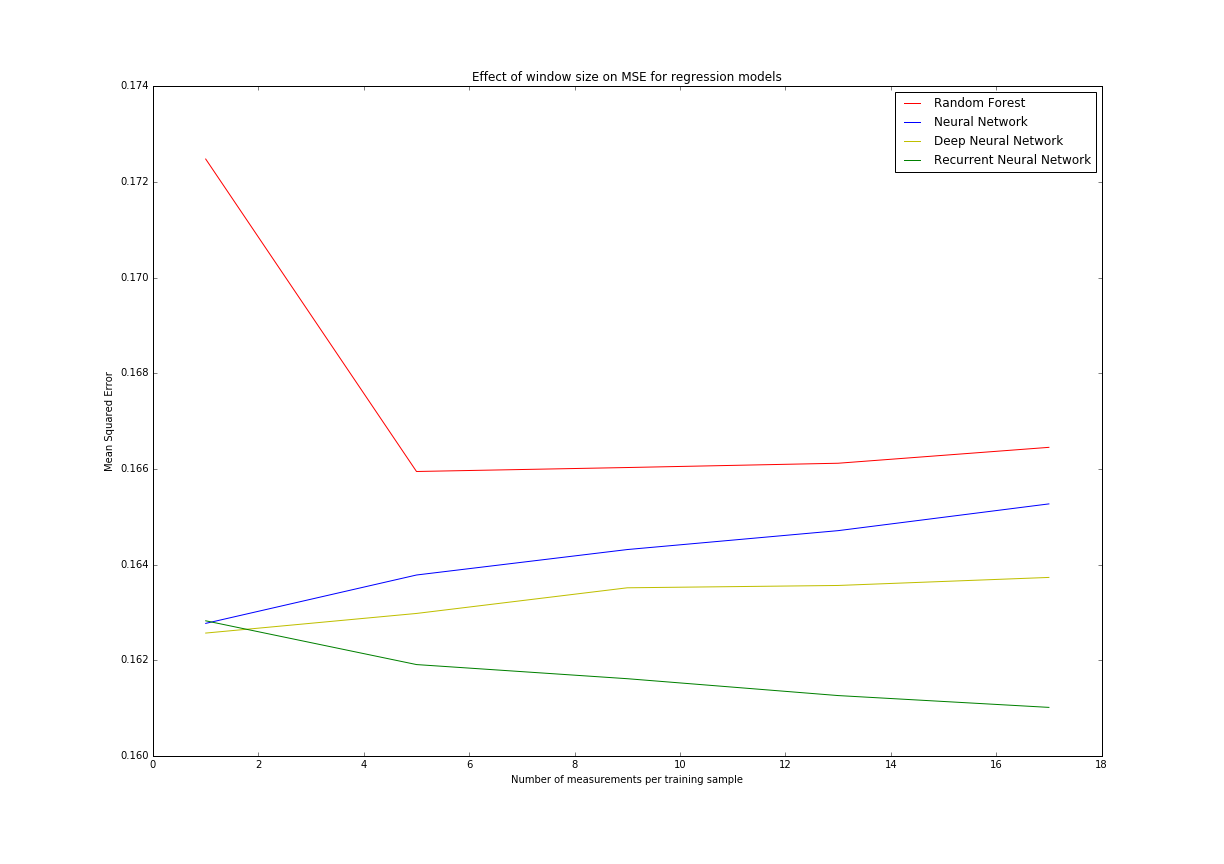
\includegraphics[height=400px, width=1.1\textwidth]{len_sequence_v_MSE}
Interestingly, besides the jump when the random forest is run on windows of length 5 instead of windows of length 1, every one of the non-recurrent models does worse as we increase the window size.  This suggests that the models struggle to train on the additional information that they are learning on.  However, the recurrent neural network's error monotonically decreases as we increase the window size - this demonstrates the power of recurrent neural nets in learning temporal associations.  

\subsection{Classification}
Given a sequence of measurements from time 0 through t, our goal is to predict the value of flag at time t + 1.  

All of these models were trained using the window method, where each training example is a sequence of 10 measurements and the result is the next value of flag.  The dataset was split 80-20 between training/validation.

\subsubsection{Random Forest Classifier (40 trees, 40 features)}
\begin{center}
\begin{tabular}{ c c c }
Window Size & Classification Rate \\
 1 & 0.760 \\
 5 & 0.818 \\
 9 & 0.803\\
 13 &  0.794\\
 17 & 0.788 
\end{tabular}
\end{center}
Confusion matrices for window size 1, 5, 9, 13, 17 respectively.  
\[
  \begin{bmatrix}
  5121 & 362 \\
  1307 & 170\\
  \end{bmatrix} 
  \begin{bmatrix}
5295  & 32 \\
1205 & 268 \\
   \end{bmatrix}
  \begin{bmatrix}
5156  & 15\\
1292 & 177\\
   \end{bmatrix}
  \begin{bmatrix}
4994  & 21\\
1310 & 155\\
   \end{bmatrix}
  \begin{bmatrix}
4839  & 20\\
1318 & 143\\
   \end{bmatrix}
\]

\subsubsection{Neural Network (1 layer, 512 nodes) }

\begin{center}
\begin{tabular}{ c c c }
Window Size & Classification Rate \\
 1 & 0.791 \\
 5 & 0.917 \\
 9 & 0.948 \\
 13 &0.954 \\
 17 &0.957 \\
\end{tabular}
\end{center}
Confusion matrices for window size 1, 5, 9, 13, 17 respectively.  
\[
  \begin{bmatrix}
  5355  &128\\
 1325  &152 \\
  \end{bmatrix} 
  \begin{bmatrix}
  [[5107 & 220] \\
 [ 346 &1127]] \\
   \end{bmatrix}
  \begin{bmatrix}
  5035 & 136 \\
 207 &1262 \\
   \end{bmatrix}
  \begin{bmatrix}
4903  &112 \\
 184 &1281\\
   \end{bmatrix}
  \begin{bmatrix}
4790  & 69 \\
199 &1262 \\
   \end{bmatrix}
\]

\subsubsection{Deep Neural Network}
\begin{center}
\begin{tabular}{ c c c }

Window Size & Classification Rate \\
 1 & 0.794 \\
 5 & 0.907 \\
 9 & 0.945 \\
 13 & 0.951 \\
 17 &0.956 \\
\end{tabular}
\end{center}
Confusion matrices for window size 1, 5, 9, 13, 17 respectively.  
\[
  \begin{bmatrix}
5382 & 101 \\
1329  &148 \\
  \end{bmatrix} 
  \begin{bmatrix}
4985  & 342\\
290 & 1183\\
   \end{bmatrix}
  \begin{bmatrix}
4994  &177\\
189  &1280\\
   \end{bmatrix}
  \begin{bmatrix}
4905 & 110\\
209 & 1256\\
   \end{bmatrix}
  \begin{bmatrix}
4773  & 86\\
190  &1271\\
   \end{bmatrix}
\]
\subsubsection{Recurrent Neural Network, window method}

\begin{center}
\begin{tabular}{ c c c }

Window Size & Classification Rate \\
 1 & 0.792 \\
 5 & 0.895 \\
 9 & 0.951 \\
 13 &0.959\\
 17 & 0.971\\

\end{tabular}
\end{center}
Confusion matrices for window size 1, 5, 9, 13, 17 respectively.  
\[
  \begin{bmatrix}
5363 & 120\\
1327  &150\\ 
   \end{bmatrix}
     \begin{bmatrix}
4861  & 466 \\
245 & 1228 \\
   \end{bmatrix}
     \begin{bmatrix}
5102  & 69 \\
256 & 1213 \\
   \end{bmatrix}
     \begin{bmatrix}
4942 &  73 \\
192  & 1273 \\
   \end{bmatrix}
     \begin{bmatrix}
4760  & 99\\
82 & 1379 \\
   \end{bmatrix}
\]

\subsubsection{Comparison}
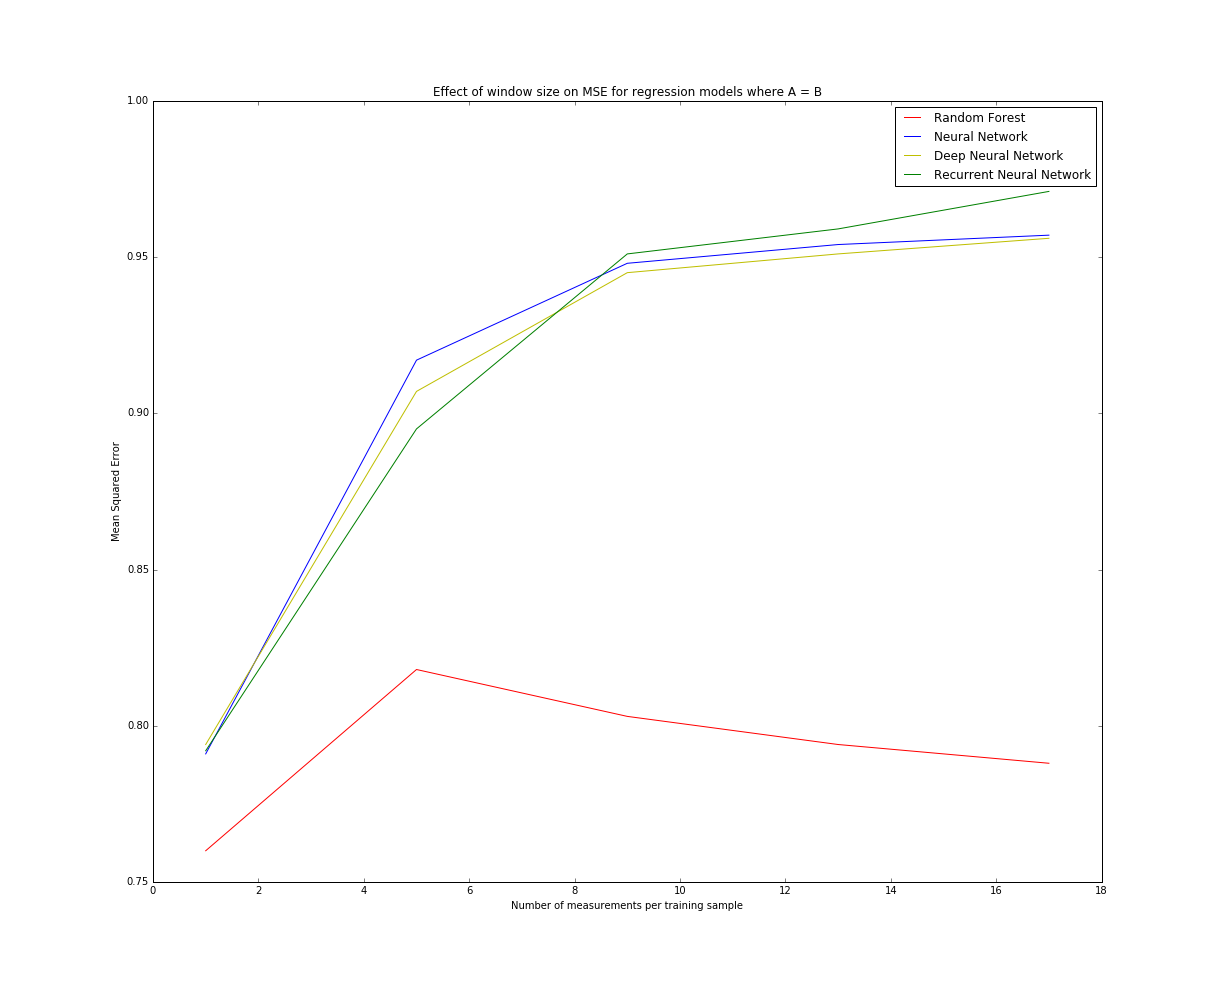
\includegraphics[height=400px, width=1.1\textwidth]{len_sequence_v_accuracy_classification}
Unlike in the regression problem, all three of the neural net model are able to increase their accuracy as the training window is increased.  The random forest is still unable to effectively make use of the new data however.  Again, the recurrent neural network performs better than the other two neural nets as we increase the window size, which we attribute to the fact that it's inherently designed to capture temporal relationships.  

\section{Acknowledgements}
I would like to thank Sahand for suggesting the interesting project and giving me advice.

 \end{document}
